The Higgs Machine learning challenge (HiggsML for short) hosted on Kaggle and sponsored by ATLAS attracted unprecedented interest from scientists in various different fields including physicists. Over 6000 people downloaded the data and by the end of the competition had uploaded over 35000 solutions among 1785 teams \cite{postRM}. The scores of all the teams are publicly available on the leader board of the HiggsML challenge on the Kaggle platform at \url{https://www.kaggle.com/c/higgs-boson/leaderboard}.

The Higgs classification problem is unique in the sense that goal of the challenge is not just to discriminate between Higgs and non-Higgs events but to provide a solution that maximizes a peculiar significance metric called the AMS ($\sigma$) based on the selection of a signal-rich region of the high-dimensional feature space. There was considerable mathematical nuance surrounding the physics of the problem. The organizers provided a training set to participants with 250K labelled events and provided an unlabelled set of 550K test events for participants to provide predictions for. The organizers reserved the weights and labels for the test events in order to prevent teams from over-fitting to the test set.  

The winning solution with the highest reported score was by Gabor Melis, a professional data scientist from Hungary. The AMS value of his solution was 3.80581. His model was an ensemble of multi-layer neural networks which used the principle of bagging. Each neural network was trained on a different subset of the full dataset creating a heterogeneous mix of networks. The output of each model was a probability estimate (usually, it is the probability that a given event belongs to the positive signal class). The prediction on an unseen sample used simple arithmetic averaging to combine the probability outputs of the bag of  models. In his own words, the most important characteristic of his model was incorporating a careful bagging procedure. His solution reflects the power of the split-train-recombine technique. Gabor published a summary account of his methodology in \cite{melis}. 

The second place winner Tim Salimans achieved a AMS score of 3.78913 on the leader board. He used a regularized greedy forest which is a variant on gradient boosting and pushes trees further away from greedy construction by adding explicit regularization terms \cite{rgf}. Further, he added and additional 30 features to the dataset taking the training time to several hours on a 4-core CPU.

XGBoost \cite{xgb} was one of the most popular choices among participants, it was rated the best single model to give strong results on the Higgs dataset. The model was used by roughly 25$\%$ of the participants and set a high performance benchmark in terms of score and speed. XGBoost is a highly scalable version of a gradient tree boosting algorithm and is available as an open source package. Part of its popularity was attributed to the fact that it provided a 10x speed scale up to the standard gradient boosting algorithm provided in python \texttt{scikit-learn}. It does so by proposing an approximate algorithm to the greedy tree construction algorithm. However, the best XGBoost model score was not in the top $10\%$ of scores achieved by participants. Many of the participants used XGBoost as part of larger ensembles with different algorithms in the mix and achieved higher scores than the single XGBoost model. This goes to show that while XGBoost is a powerful model, there was room for improving performance using different types of ensembles.  

The one thing that is apparent from this study is that a lot of the models that bagged top scores were overkill in terms of their architecture and computational sophistication. Gabor Melis trained his ensemble of neural networks on a GTX Titan GPU where training a single 3-layer network took 10 minutes. As a comparison the solution provided in this thesis runs on a 4-core CPU machine and the entire model trains in under 30 mins. The winning scores are in table \ref{leader}, the boosted extremely random trees (BXT) algorithm proposed in this thesis achieves an AMS score of 3.793$\sigma$. 

\begin{figure}
\centering
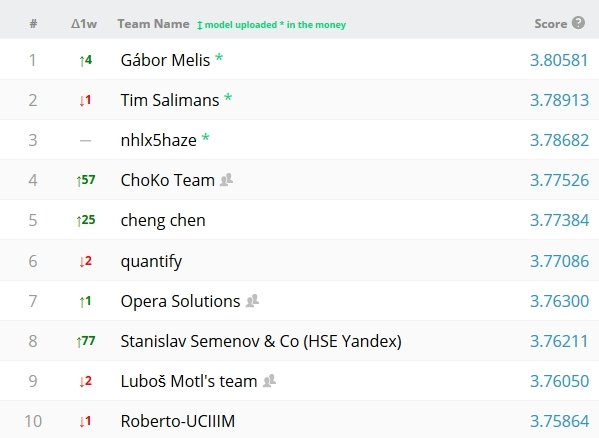
\includegraphics[width=0.7\textwidth]{images/leaderboard_final.jpg}
\caption{Leading solutions to the HiggsML Challenge (2014)}
\label{leader}
\end{figure}

